% ****** Start of file apssamp.tex ******
%
%   This file is part of the APS files in the REVTeX 4.1 distribution.
%   Version 4.1r of REVTeX, August 2010
%
%   Copyright (c) 2009, 2010 The American Physical Society.
%
%   See the REVTeX 4 README file for restrictions and more information.
%
% TeX'ing this file requires that you have AMS-LaTeX 2.0 installed
% as well as the rest of the prerequisites for REVTeX 4.1
%
% See the REVTeX 4 README file
% It also requires running BibTeX. The commands are as follows:
%
%  1)  latex apssamp.tex
%  2)  bibtex apssamp
%  3)  latex apssamp.tex
%  4)  latex apssamp.tex
%
\documentclass[%
 preprint,
%superscriptaddress,
%groupedaddress,
%unsortedaddress,
%runinaddress,
%frontmatterverbose, 
%preprint,
%showpacs,preprintnumbers,
%nofootinbib,
%nobibnotes,
%bibnotes,
 amsmath,amssymb,
 aps,
%pra,
%prb,
%rmp,
%prstab,
%prstper,
%floatfix,
]{revtex4-1}

\usepackage{graphicx}% Include figure files
\usepackage{dcolumn}% Align table columns on decimal point
\usepackage{bm}% bold math
\usepackage{hyperref}% add hypertext capabilities
%\usepackage[mathlines]{lineno}% Enable numbering of text and display math
%\linenumbers\relax % Commence numbering lines

%\usepackage[showframe,%Uncomment any one of the following lines to test 
%%scale=0.7, marginratio={1:1, 2:3}, ignoreall,% default settings
%%text={7in,10in},centering,
%%margin=1.5in,
%%total={6.5in,8.75in}, top=1.2in, left=0.9in, includefoot,
%%height=10in,a5paper,hmargin={3cm,0.8in},
%]{geometry}

\usepackage{braket} % Allows for Dirac notation
%\usepackage{subcaption}

\newcommand{\veff}{\hat{V}_{12,\text{eff}}}
\newcommand{\rhozero}{\rho_{\text{I}=0}}
\newcommand{\rhoone}{\rho_{\text{I}=1}}

\newcommand{\yukawa}[1]{\frac{e^{-m_\pi |#1|}}{4\pi |#1|}}
\newcommand{\yukawadimless}[1]{\frac{e^{-m_\pi #1}}{m_\pi #1}}
\newcommand{\yukawanoabs}[1]{\frac{e^{-m_\pi #1}}{4\pi #1}}

\newcommand{\rot}{\vec{r}_{12}}
\newcommand{\rotp}{\vec{r}_{12}\!\!'}

\newcommand{\taudot}{\vec{\tau}_1\cdot\vec{\tau}_2}
\newcommand{\sigmadot}{\vec{\sigma}_1\cdot\vec{\sigma}_2}

\newcommand{\lvec}[1]{\reflectbox{\ensuremath{\vec{\reflectbox{\ensuremath{#1}}}}}}

\newcommand{\threej}[6]{ \begin{pmatrix}
  #1 & #2 & #3 \\
  #4 & #5 & #6 
 \end{pmatrix}}

\newcommand{\sixj}[6]{ \begin{Bmatrix}
  #1 & #2 & #3 \\
  #4 & #5 & #6 
 \end{Bmatrix}}

\newcommand{\ninej}[9]{ \begin{Bmatrix}
  #1 & #2 & #3 \\
  #4 & #5 & #6 \\
  #7 & #8 & #9
 \end{Bmatrix}}

\begin{document}

\preprint{APS/123-QED}

\title{Energy spectra of two interacting fermions with spin-orbit coupling in a harmonic trap}% Force line breaks with \\
%\thanks{A footnote to the article title}%

\author{Cory D. Schillaci}
\email{schillaci@berkeley.edu}
\affiliation{%
Department of Physics, University of California, Berkeley, California 94720, USA
}%

\author{Thomas C. Luu}%
\email{
t.luu@fz-juelich.de
}
\affiliation{
Institute for Advanced Simulation, Institut f\"{u}r Kernphysik and J\"{u}lich Center for Hadron Physics, Forschungszentrum J\"{u}lich, D-52425 J\"{u}lich, Germany
}
%\affiliation{Institut f\"{u}r Kernphysik and J\"{u}lich Center for Hadron Physics,
%Forschungszentrum J\"{u}lich, D-52425 J\"{u}lich, Germany}%Lines break automatically or can be forced with \\

\date{\today}% It is always \today, today,
             %  but any date may be explicitly specified

\begin{abstract}
We explore the two body spectra of spin-$1/2$ fermions in isotropic harmonic traps with external spin-orbit potentials and short range two body interactions. Using a truncated basis of total angular momentum eigenstates, nonperturbative results are presented for experimentally realistic forms of the spin-orbit coupling: pure Rashba, equal parts Rashba and Dresselhaus, and Weyl type spin-orbit couplings. The technique is easily adapted to bosonic systems and other forms of spin-orbit coupling.
%Matrix elements are calculated in a basis of total angular momentum eigenstates to best expose the underlying symmetries 
\end{abstract}

%\pacs{Valid PACS appear here}% PACS, the Physics and Astronomy
                             % Classification Scheme.
%\keywords{Suggested keywords}%Use showkeys class option if keyword
                              %display desired
\maketitle

%\tableofcontents

\section{\label{sec:level1}Introduction}

Cold atomic gases with spin-orbit coupling (SOC) have recently been an area of intense interest because of the potential to simulate interesting physical systems with precisely tunable interactions \cite{nature11841}. In condensed matter physics, spin-orbit couplings are essential for many exotic systems such as topological insulators \cite{das2013engineering,PhysRevLett.105.255302}, the quantum spin hall effect\cite{nature12185}, and spintronics \cite{RevModPhys.76.323}. The experimental setup which induces spin-orbit coupling is intimately related to simulation of synthetic gauge fields \cite{RevModPhys.83.1523,hamner2014dicke,Lin:2009zzb,Bermudez:2011db}. Because they are parity-violating like the weak force, spin-orbit couplings feature prominently in nuclear physics where they are an essential ingredient in realistic effective nuclear forces. Atomic gases provide an excellent testing ground both to explore universal behaviour of these real life systems and to create new types of spin-orbit coupling which are not yet known to exist (or have no solid-state analog) in other materials but are interesting in their own right. Further, these experiments can be performed in an environment with little to no defects or impurities.

Spin-orbit coupling was first realized in a Bose condensate of $^{87}$Rb \cite{nature09887} and extended shortly after to Fermi gases of $^{40}$K \cite{PhysRevLett.109.095301} and $^6$Li \cite{PhysRevLett.109.095302}. These spin-orbit interactions are `synthetic' in the sense that a subset of the hyperfine states stand in as virtual spin states.   The application of these couplings is equivalent to applying an external electric or magnetic force on spin-states, but with particles that are neutral in charge \cite{Lin:2011,PhysRevLett.107.255301}.  A particularly interesting consequence of these atomic systems is the possibility of studying bosonic systems with synthetic spin-$1/2$ spin orbit interactions \cite{PhysRevA.68.063612,nature09887}.   It has also been conjectured that these systems could be used to physically simulate lattice gauge theories \cite{Bermudez:2010da,Mazza:2011kf}.  Spin-orbit couplings in solid state systems arise in 2D systems (Rashba and Dresselhaus types, described in sect. \ref{sec:Hamiltonian}), but recently an experimental setup has been proposed that can simulate the Weyl type SOC which is fundamentally three dimensional \cite{PhysRevLett.108.235301}.

Calculations of few-atom systems in a trap undergoing SOC are also being developed.  For example, the spectrum of particles within a trap with an external SOC of the Weyl type (but no relative interaction) has been theoretically determined \cite{anderson2013}. The Rashba SOC with two-particle systems interacting via short-ranged interactions have also been investigated perturbatively, where it was shown that the leading order behavior of the SOC was independent of the scattering as long as the scattering length is equal for all channels \cite{PhysRevA.89.033606}.  In one dimension, the spectrum for this type of system has been calculated when the SOC consists of equal parts Rashba and Dresselhaus interactions \cite{guan2014energy}.  For three particles in a trap under the influence of SOC, a new type of universality is conjectured to occur for bound trimers with negative scattering length \cite{PhysRevLett.112.013201}.  In all these calculations, the emergent spectrum is rich and complex, offering new insights in many-body behavior.

Our objective is to provide some insight into the few-body physics of Fermi gases with spin-orbit interactions in the presence of trapping potentials and two-body interactions, which are necessarily present in cold-atom experiments. Our approach is to numerically diagonalize the Hamiltonian within a suitably truncated basis. Eigenstates of the interacting Hamiltonian without SOC are used for the basis. Section \ref{sec:Hamiltonian} introduces the specific forms of spin-orbit coupling and two-body interactions which we consider. The general method is detailed in Section \ref{sec:Weyl} for the simplest SOC.  In the remaining sections \ref{sec:Rashba}-\ref{sec:R=D} we study the spectra of additional spin-orbit couplings in order of increasing computational complexity.

\section{\label{sec:Hamiltonian}Hamiltonian for Spin-orbit Couplings with Contact Interactions}

In this paper we simply refer to our systems by their `spin' degrees of freedom and use the standard notation for spin quantum numbers. we consider three different types of spin-orbit coupling (SOC). The form of spin-orbit coupling realized in experiments is a linear combination of the Rashba \cite{0022-3719-17-33-015} and linear Dresselhaus \cite{PhysRev.100.580} types,
\begin{align}
V_{R}&=\alpha_R (\sigma_x k_y-\sigma_y k_x) \label{eq:Rashba},\\
V_{D}&=\alpha_D (\sigma_x k_y+\sigma_y k_x) \label{eq:Dresselhaus},
\end{align} 
which were originally recognized in two-dimensional solid state systems. In a two-dimensional system, these form a complete basis for spin-orbit couplings linear in momentum. Note that some references use the alternate definitions $V_R\propto  (\sigma_x k_x+\sigma_y k_y) $ and $V_D\propto  (\sigma_x k_x-\sigma_y k_y) $ which are equivalent up to a pseudospin rotation.  For solids, these parity violating interactions are only allowed in the absence of inversion symmetries. Rashba type SOC typically arises in the presence of applied electric fields or in 2D subspaces such as the surfaces of materials where the boundary breaks the symmetry. Dresselhaus couplings were first studied in the context of bulk inversion asymmetry, when the internal structure leads to gradients in the microscopic electric field. 

%The simplest scenario for which the Rashba SOC arises is the case of electrons in the presence of a static electric field. Electrons moving with respect to the lab frame will experience a magnetic field due to Lorentz invariance, which leads to a velocity dependent Zeeman effect of the form \eqref{eq:Rashba}. Dresselhaus type interactions ???

To date, experiments have only produced SOC potentials in which the Rashba and Dresselhaus terms appear with equal strength, also known as the ``persistent spin-helix symmetry point'' \cite{PhysRevLett.97.236601}, 
\begin{equation}
\label{eq:R=D}
V_{R=D}=\alpha_{R=D}\sigma_x k_y.
\end{equation} 
After a rotation, this potential can be seen as a unidirectionall coupling of the pseudo-spin and momentum along a single axis. A proposal for tuning the ratio $\alpha_R/\alpha_D$ has been given in \cite{PhysRevA.84.025602}.  An experimental setup which gives the simple three-dimensional Weyl coupling,
\begin{equation}\label{eq:Weyl}
V_{W}=\alpha_W \vec{k}\cdot\vec{\sigma},
\end{equation}
has also been proposed in \cite{PhysRevLett.108.235301} and \cite{PhysRevLett.111.125301}. %The single particle energy levels for this coupling were found numerically in \cite{0953-4075-46-13-134003}. 

In the following sections we calculate the spectra of two particles with a short-range two-body interaction, an isotropic harmonic trapping potential and spin-orbit coupling. The single particle Hamiltonian is,
\begin{equation}\label{eq:shortRangeInteraction}
H_1=\frac{\hbar^2 k^2}{2m}+\frac{1}{2}m\omega^2 r^2 + V_{SO}.
\end{equation}
For the spin-orbit term $V_{SO}$, we consider equal Rashba and Dresselhaus \eqref{eq:R=D}, pure Rashba \eqref{eq:Rashba}, and Weyl \eqref{eq:Weyl} spin-orbit couplings  because these are generally considered to be experimentally feasible.

We assume that the range of interaction between particles is small compared to the size of the oscillator well.  The relative interaction between the particles can then be approximated as a regulated s-wave contact interaction, which in momentum space (as a function of relative momentum) is given by
\begin{equation}
\frac{4\pi \hbar^2}{m}a(\Lambda)\ .
\end{equation}
Here the argument $\Lambda$ refers to some cutoff scale and $a(\Lambda)$ is some function of the cutoff and physical scattering length $a_{\text{phys}}$.  The exact form of $a(\Lambda)$ depends on the type of regulator used and is not relevant for this work; the only constraint is that $a(\Lambda)$ reproduce the physical scattering length given by the scattering $T$-matrix at threshold, $T(E=0)=4\pi\hbar^2 a_{\text{phys}}/m$ \cite{taylor2000}. In the limit $\Lambda\rightarrow \infty$ the spectrum of two particles in an oscillator well (without external spin-orbit interaction) was solved by Busch et al. \cite{Busch} using the method of pseudo-potentials.  In reference  \cite{Luu:2006xv} the solution for general $\Lambda$ was given using a Gaussian regulator, which in the limit $\Lambda\rightarrow\infty$ recovered the Busch et al. solution.  For our work below we use the eigenstates and eigenvalues given by  \cite{Busch}.

\section{\label{sec:Weyl}Weyl coupling}
We tackle the Weyl form first because of its mathematical and numerical simplicity. In the absence of the two-body interaction, this problem was treated by reference \cite{0953-4075-46-13-134003}. Our approach is to determine the matrix elements of the SOC in an appropriate basis. The eigenvalue is then solved numerically at the desired precision by choosing an appropriately large truncated basis of harmonic oscillator eigenstates.

As usual, the two-body problem is best approached in the dimensionless Jacobi coordinates,
\begin{equation}
R=\frac{r_1+r_2}{\sqrt{2}b}, \qquad r=\frac{r_1-r_2}{\sqrt{2}b},
\end{equation}
and the corresponding conjugate momenta $q,Q$ representing the relative and total momenta. For an isotropic harmonic oscillator, distances can be expressed in terms of the ground state length scale $b=\sqrt{\hbar/m\omega}$ and energies will be similarly measured in units of $E_0=\hbar\omega$. We also define the spin operators
\begin{equation}
\vec{\sigma}=\vec{\sigma}_1-\vec{\sigma}_2, \qquad \vec{\Sigma}=\vec{\sigma}_1+\vec{\sigma}_2.
\end{equation}

With these definitions, the two-body Hamiltonian can be separated into relative and center of mass (CM) parts,
\begin{equation}\label{eq:WeylHamiltonian}
\frac{1}{\hbar\omega}H=\left(h_{0,\text{rel}}+\frac{\tilde{\alpha}_W}{\sqrt{2}} \vec{q}\cdot\vec{\sigma} + \sqrt{2}\pi \tilde{a}(\Lambda) \delta^{(3)}(r)\right)+\left(h_{0,\text{CM}}+\frac{\tilde{\alpha}_W}{\sqrt{2}} \vec{Q}\cdot\vec{\Sigma} \right)
\end{equation}
Notably, the spin-orbit coupling appears in both terms. The tilde over the coupling constants indicates that they are dimensionless, related to the original coupling constants by dividing out the oscillator length (e.g. $\tilde{\alpha}=\alpha/b$).

Eigenstates of two particles with a short range interaction in a harmonic oscillator trapping potential form a convenient basis for these calculations. These basis functions were first derived in \cite{Busch} for the isotropic case considered here, and the more general case of an anisotropic trap has been explored by \cite{PhysRevA.74.022712}. We choose the particular coupling scheme of angular momentum eigenstates,
\begin{equation}\label{eq:basisStates}
\ket{n(ls)j;NL;(jL)J},
\end{equation}
which simplify the matrix elements for the relative coordinate operators. The total spin of the two spin-$1/2$ particles is denoted by $s = s_1 + s_2$ and may be either 0 or 1. Total spin $s$ is first coupled with $l$ to make angular momentum $j$, which is then recoupled with the CM angular momentum $L$ to make the state's total angular momentum $J$. Because all terms in the Hamiltonian \eqref{eq:WeylHamiltonian} are scalars, the interaction is independent of $J_z$ and so we omit this quantum number for clarity. Due to Pauli exclusion, $l + s$ must be even to enforce antisymmetry under exchange of the particles.

For $l\neq0$ the states \eqref{eq:basisStates} are identical to the well known harmonic oscillator, with $n,l$ indicating the relative HO quantum numbers, and $N,L$ the center of mass HO quantum numbers. We use the convention that $n,N=0,1,2,\dots$, therefore $E=2n+l+2N+L+3$. The short range interaction \eqref{eq:shortRangeInteraction} modifies the $l=0$ states and their spectrum. The principle relative quantum number $n$ for these states is obtained by solving the transcendental equation
\begin{equation}\label{eq:eigenvalueEqn}
\sqrt{2}\frac{\Gamma(-n)}{\Gamma(-n-1/2)}=\frac{1}{a}
\end{equation}
and is no longer integer valued. For the relative coordinate part of the $l=0$ wave function,
\begin{align}
\phi(r)&=\frac{1}{2\pi^{3/2}}A(n)\Gamma(-n)U(-n,3/2,r^2)e^{-r^2/2}, \label{eq:BuschWF}\\
A(n)&=\left(\frac{\Gamma(-n)[\psi_0(-n)-\psi_0(-n-1/2)]}{8 \pi^2 \Gamma(-n-1/2)}\right)^{-1/2},
\end{align}
where $U(a,b,x)$ is Kummer's confluent hypergeometric function and $\psi_0(x)=\Gamma'(x)/\Gamma(x)$ is the digamma function. A derivation of the normalization factor $A(n)$ is given in the Appendix.

Standard angular momentum algebra can be used to determine the matrix elements of the two spin-orbit coupling terms; we follow the conventions of \cite{Edmonds}. For Weyl SOC coupling of two spin-$1/2$ fermions, the matrix elements of the coupling in the relative momentum are
\begin{equation}\label{eq:WeylRel}\begin{split}
\bra{n'(l's')j';N'L';(j'L')J'}\vec{q}&\cdot\vec{\sigma} \ket{n(ls)j;NL;(jL)J} = \\
&\delta_{N,N'}\delta_{L,L'}\delta_{j,j'}\delta_{J,J'}(-1)^{l+s'+j}\frac{3}{\sqrt{2}}\sixj{j}{s'}{l'}{1}{l}{s} (s'-s)\braket{n'l' || q || n l}.
\end{split}
\end{equation}
This is nonzero only if $s\neq s'$, i.e. the operator changes the total spin of the two particles as expected for a parity violating potential. The relative momentum term in the Weyl SOC operator connects states with different parity while preserving the antisymmetry of the state by also changing the relative angular momentum by $\pm1$, leaving $l+s$ even. 

Between states with $l,l'\neq0$, reduced matrix elements of the momentum operator are calculated between pure harmonic oscillator states,
% Should do away with some constants in favor of the 3-j coefficient?
\begin{align}
\braket{n'l' || q || n l}=&(-1)^{l'}(-1)^{\frac{l+l'+1}{2}}\sqrt{\frac{2(2l+1)(2l'+1)}{(l+l'+1)}}\braket{n'l'0| (-i \nabla_0) | n l 0} \\
\begin{split} =& i(-1)^{l}\sqrt{\frac{l+l'+1}{2}}\sqrt{n!n'!\Gamma(n+l+3/2)\Gamma(n'+l'+3/2)} \\ 
&\times\sum_{m,m'=0}^{n,n'} \left\{
     \begin{array}{lr}
       \frac{(-1)^{m+m'}\left[2m\Gamma\left(m+m'+1+\frac{l+l'}{2}\right)-\Gamma\left(m+m'+1+\frac{l+l'}{2}\right)\right]}{m!m'!(n-m)!(n'-m')!\Gamma(m+l+3/2)\Gamma(m'+l'+3/2)} & \text{if}\: l'=l-1 \\
        \frac{(-1)^{m+m'+1}\left[(2m+2l+1)\Gamma\left(m+m'+1+\frac{l+l'}{2}\right)-\Gamma\left(m+m'+1+\frac{l+l'}{2}\right)\right]}{m!m'!(n-m)!(n'-m')!\Gamma(m+l+3/2)\Gamma(m'+l'+3/2)} & \text{if}\: l'=l+1 \\
       0 & \text{otherwise}
     \end{array}
   \right.
   \end{split}
\end{align}
If $l=1$ and $l'=0$ or vice versa, reduced matrix elements between one of modified wave function of the form \eqref{eq:BuschWF} and one pure harmonic oscillator state are needed. These are given by,
\begin{align}
\braket{n l=0 || q || n' l'=1}=-i A(n) \sqrt{\frac{\Gamma(n'+5/2)}{2\pi^3 n'!}}\frac{2n-2n'-1}{2(n'-n)(1+n'-n)},
\end{align}
and its Hermitian conjugate.

Our choice of basis makes the CM matrix elements \eqref{eq:WeylRel} simple at the cost of complicating the center-of-mass term. We take the approach of expanding the states \eqref{eq:basisStates} in the alternate coupling scheme,
\begin{equation}\label{eq:basisStates2}
\ket{n(ls)j;NL;(jL)J}=(-1)^{l+s+L+J}\sqrt{2j+1}\sum_{\mathcal{J}}\sqrt{2\mathcal{J}+1}\sixj{l}{s}{j}{L}{J}{\mathcal{J}}\ket{nl;N(Ls)\mathcal{J};(l\mathcal{J})J}.
\end{equation}
Using this notation, the matrix elements can be written
\begin{equation}\begin{split}
\bra{n'(l's')j';N'L';(j'L')J'}&\vec{Q}\cdot\vec{\Sigma} \ket{n(ls)j;NL;(jL)J} = \delta_{n,n'}\delta_{l,l'}\delta_{J,J'}\delta_{s,1}\delta_{s1,1}   6 (-1)^{L} \\
&\hspace{-1cm}\times\braket{N'L'|| \vec{Q} || NL} \sum_{\mathcal{J}}(-1)^\mathcal{J} (2\mathcal{J}+1)\sixj{l}{1}{j'}{L'}{J}{\mathcal{J}}\sixj{l}{1}{j}{L}{J}{\mathcal{J}}\sixj{\mathcal{J}}{1}{L'}{1}{L}{1}.
\end{split}
\end{equation}
Again, the reduced matrix element of the CM momentum changes the parity by connecting states with $\Delta L=\pm1$. Matrix elements are non-zero only for $\Delta s=0$ because the antisymmetry of the wave function depends on $l$ which does not change. We also note that the CM term does not affect states with singlet spin wave functions ($s=0$).


\begin{figure}
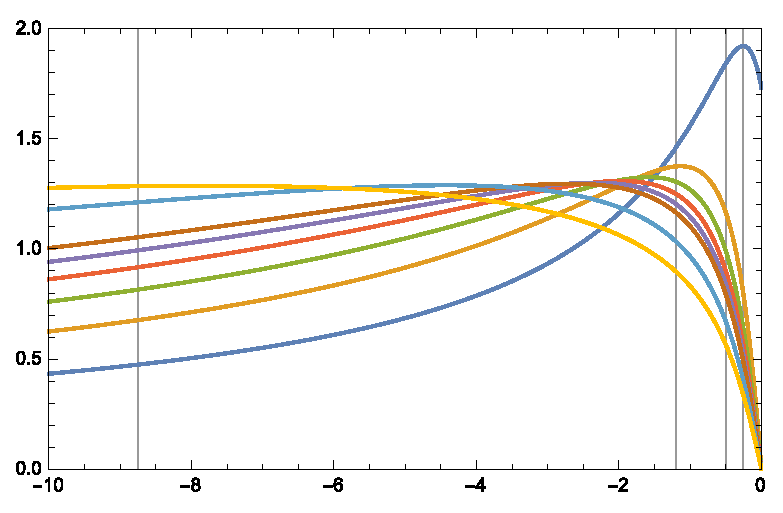
\includegraphics[height=0.28\linewidth]{Figures/sigma_dot_q_mat_elts}\nobreak
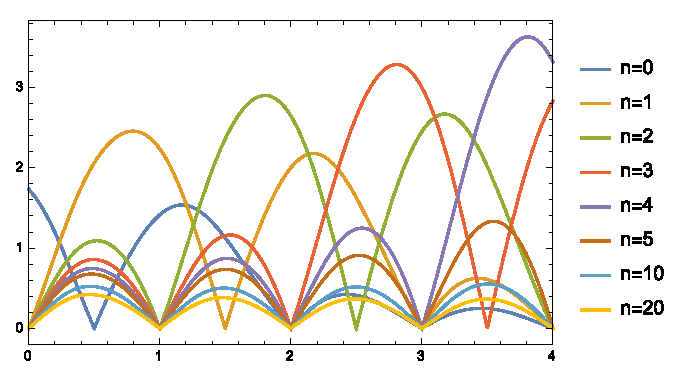
\includegraphics[height=0.278\linewidth]{Figures/sigma_dot_q_mat_elts2}
\caption{\label{fig:matrixElts}Absolute value of the matrix elements $|\bra{n'(11)0;00;(00)0}\vec{\sigma}\cdot\vec{q}\ket{n(00)0;00;(00)0}|$ between the ground state and $l=1$ excited states. The horizontal axis is the principal quantum number of the ground state obtained from solving  \eqref{eq:eigenvalueEqn}. From left to right, the vertical lines on the negative axis indicate the values obtained for $a=1/4$, $a=1$, $a=\pm\infty$, and $a=-1$ respectively.} 
\end{figure}

Using these matrix elements, we calculated the spectrum of the two interacting particles with Weyl spin-orbit coupling. Our calculations are performed by numerically diagonalizing in a truncated basis of the harmonic oscillator states \eqref{eq:basisStates}, where a cutoff $2N+L+2n+l+3\leq E_{max}$ is set high enough that the eigenvalues of the matrix have converged to the desired accuracy.  This approach converges well only when the ground state energy is not too low. In particular, for $a$ positive but very small the principal quantum number of the ground state is increasing from negative infinity. For this regime, the matrix elements involving an $l=0$ state are actually larger when connecting to an $l=1$ state with moderately high $n$ than they are for small $n$ (in Section \ref{sec:Rashba} we show that relative coordinate excitations dominate the spectrum for the ground state). This situation is shown in the left panel of Figure \ref{fig:matrixElts}. For excited states, $n$ is always positive and the dominant matrix elements are always with the most similar harmonic oscillator states.

\begin{figure}
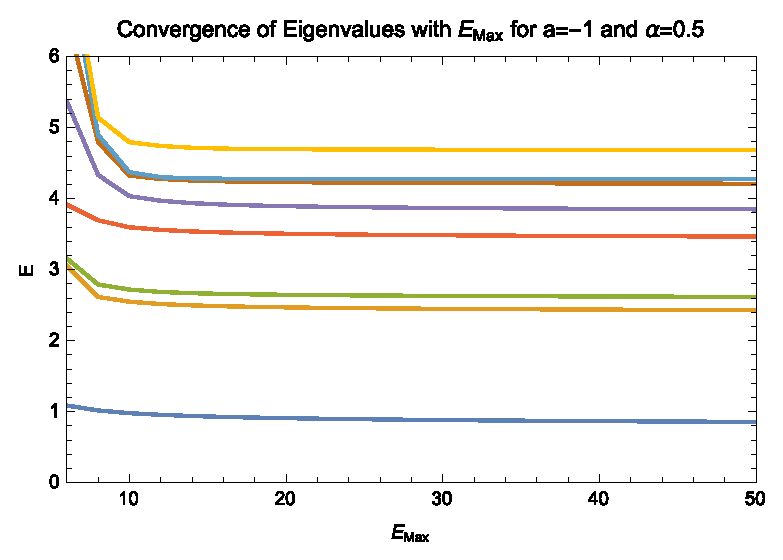
\includegraphics[width=0.5\linewidth]{Figures/WeylConvM1}\nobreak
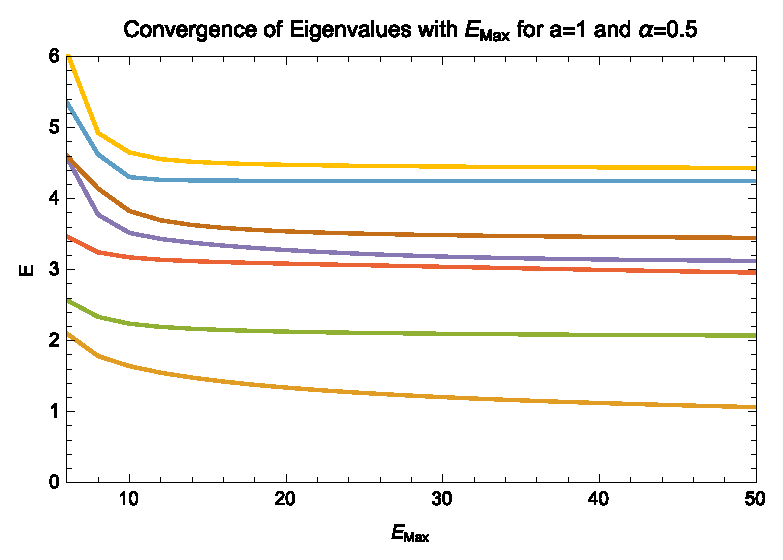
\includegraphics[width=0.5\linewidth]{Figures/WeylConvP1}
\caption{\label{fig:WeylConvergence} Convergence of the eigenvalues in the truncated basis with increasing $E_{max}$.} 
\end{figure}


\begin{figure}
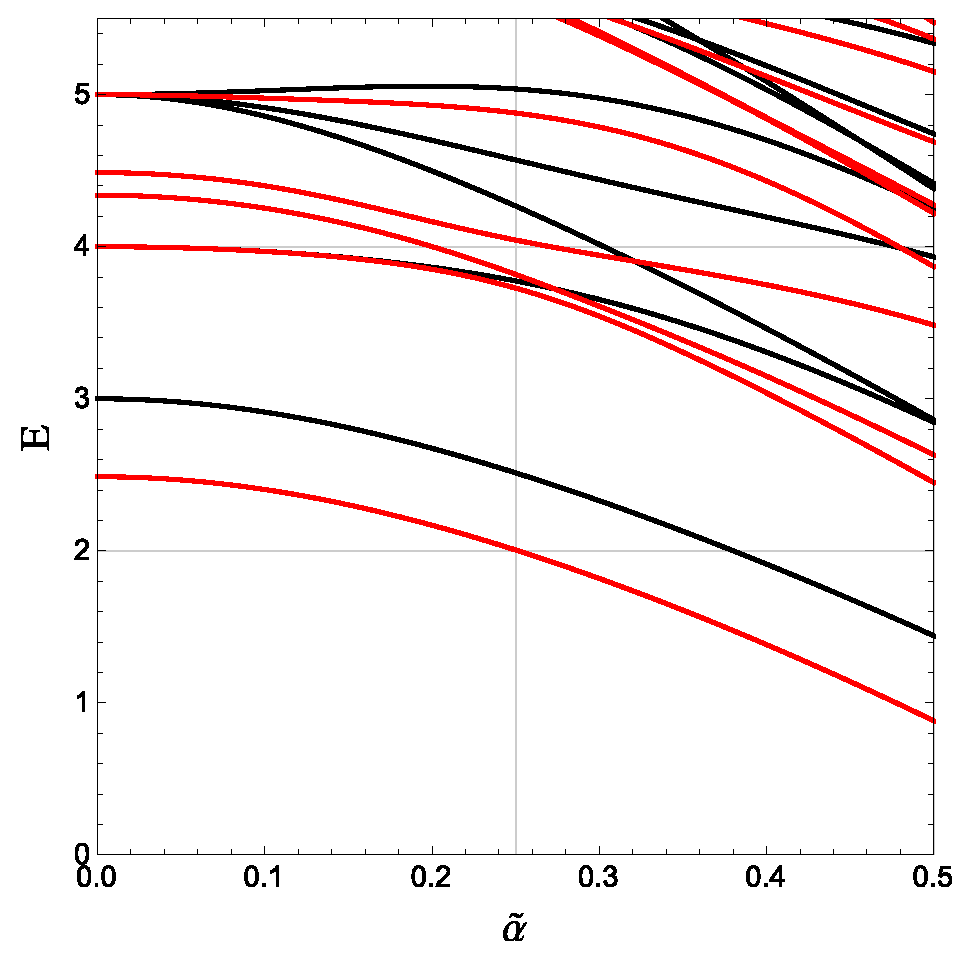
\includegraphics[width=0.5\linewidth]{Figures/Weyla0am1}\nobreak
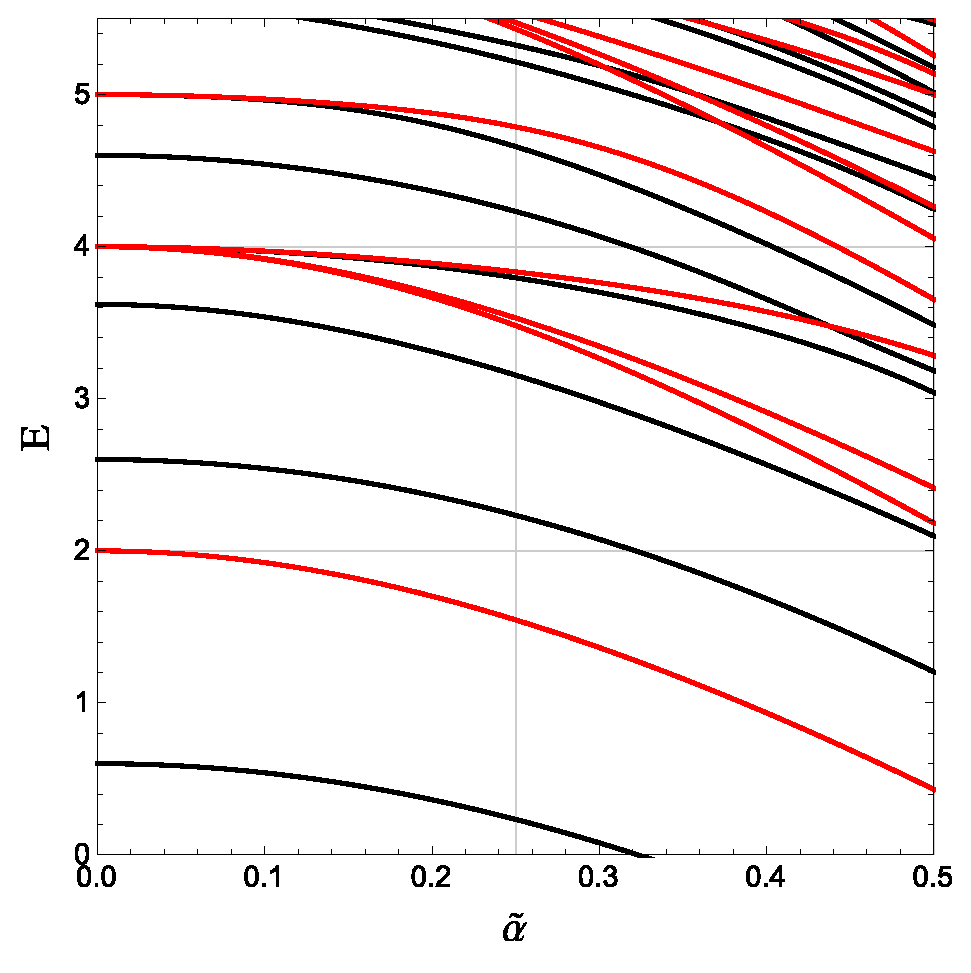
\includegraphics[width=0.5\linewidth]{Figures/Weyla1aInf}
\caption{\label{fig:WeylSpectrum} Spectrum of states with total angular momentum $J=0$ for the Hamiltonian \eqref{eq:WeylHamiltonian}. The left figure shows the energies without the two-body interaction, i.e. $\tilde{a}_W=0$ (black), and with negative scattering length $\tilde{a}_W=-1$ (red). The right figure shows the results for a positive scattering scattering length $\tilde{a}_W=1$ (black) and in the unitary limit $\tilde{a}_W\rightarrow\infty$ (red).} 
\end{figure}


As a result, convergence of the ground state is actually more difficult than that for nearby excited states. Furthermore, our approach gives the best convergence when $a$ is not small and positive. We compare the convergence of the $a=-1$ and $a=1$ spectra in Figure \ref{fig:WeylConvergence} to demonstrate how the matrix truncation plays out in practice. The actual energy spectrum is shown in Figure \ref{fig:WeylSpectrum}. We estimate that all of the energies shown have converged to within no more than $.01\hbar\omega$. For $a=0$, the convergence is to within $10^{-5}\hbar\omega$.

\section{\label{sec:Rashba}The Pure Rashba SOC}

In order to find the matrix elements of the pure Rashba coupling given in \eqref{eq:Rashba}, we first note that it can be written as a spherical tensor,
\begin{equation}
V_{R}=i\sqrt{2}\:\alpha_R \left[ k \otimes \sigma \right]_{10}.
\end{equation}
We therefore have the two-body Hamiltonian,
\begin{equation}\label{eq:RashbaHamiltonian}
\frac{1}{\hbar\omega}H=\left(h_{0,\text{rel}}+i \tilde{\alpha}_R  \left[ \vec{q} \otimes \vec{\sigma} \right]_{10} + \sqrt{2}\pi \tilde{a}(\Lambda) \delta^{(3)}(r)\right)+\left(h_{0,\text{CM}}+i \tilde{\alpha}_R [ \vec{Q}\otimes \vec{\Sigma} ]_{10} \right).
\end{equation}

Because the spin orbit coupling is now a $k=1$ tensor rather than a scalar operator, total angular momentum $J$ is no longer conserved. Additionally, the matrix elements now depend on the quantum number $J_z$ (which is conserved). For the relative coordinate part of the SOC, some algebra gives
\begin{equation}\begin{split}
&\bra{n'(l's')j';N'L';(j'L')J'J'_z}  [ \vec{q} \otimes \vec{\sigma} ]_{10}  \ket{n(ls)j;NL;(jL)JJ_z} =6 i (-1)^{J+J'-J'_z+j'+L+1}\delta_{N,N'}\delta_{L,L'}\delta_{J_z,J'_z} \\
 &\times\sqrt{(2J+1)(2J'+1)(2j+1)(2j'+1)} \threej{J'}{1}{J}{-J_z}{0}{J_z} \sixj{j'}{J'}{L}{J}{j}{1}
 \renewcommand{\arraystretch}{0.9}
 \ninej{\hphantom{l}l'\hphantom{l}}{\hphantom{l}l\hphantom{l}}{\hphantom{l}1\hphantom{l}}{s'}{s}{1}{j'}{j}{1} (s'-s) \braket{n'l' || q || n l},
\end{split}
\end{equation}
This expression presents somewhat more numerical difficulty than \eqref{eq:WeylRel} because of the dependence on many Wigner $j$ symbols which become expensive for larger angular momentum quantum numbers.

For the CM part of the Hamiltonian we again expand the basis states in the alternate coupling scheme to obtain the matrix elements,
\begin{equation}\begin{split}
&\bra{n'(l's')j';N'L';(j'L')J'J'_z} [ \vec{Q} \otimes \vec{\Sigma} ]_{10}  \ket{n(ls)j;NL;(jL)JJ_z} = \delta_{n,n'}\delta_{l,l'}\delta_{J_z,J'_z}\delta_{s,1}\delta_{s',1} \\
 &\quad\times 6 i \sqrt{2}(-1)^{J+J'-J'_z+l} \sqrt{(2J+1)(2J'+1)(2j+1)(2j'+1)} \threej{J'}{1}{J}{-J_z}{0}{J_z}  \braket{N' L' || Q || N L} \\ 
 &\quad\times\sum_{\mathcal{J},\mathcal{J}'} (-1)^\mathcal{J}(2\mathcal{J}+1)(2\mathcal{J}'+1)\sixj{l}{1}{j'}{L'}{J'}{\mathcal{J}'}\sixj{l}{1}{j}{L}{J}{\mathcal{J}}\sixj{\mathcal{J}'}{J'}{l}{J}{\mathcal{J}}{1}
 \renewcommand{\arraystretch}{0.9}
 \ninej{\hphantom{l}L'\hphantom{l}}{\hphantom{l}L\hphantom{l}}{\hphantom{l}1\hphantom{l}}{1}{1}{1}{\mathcal{J}'}{\mathcal{J}}{1} .
\end{split}
\end{equation}
Similarly to the relative term, the Wigner 9-$j$ symbol and the double summation  increase the computational cost of evaluating matrix elements over the Weyl case.

\begin{figure}
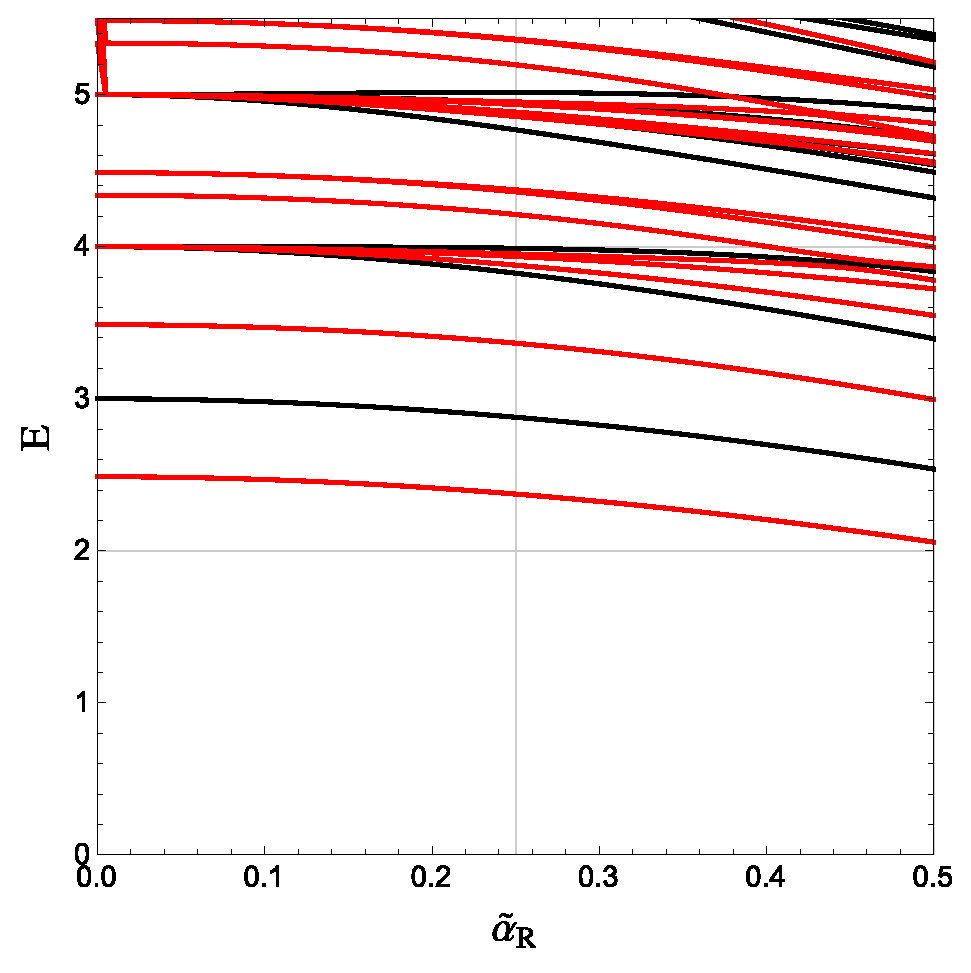
\includegraphics[width=0.5\linewidth]{Figures/Rashbaa0am1}\nobreak
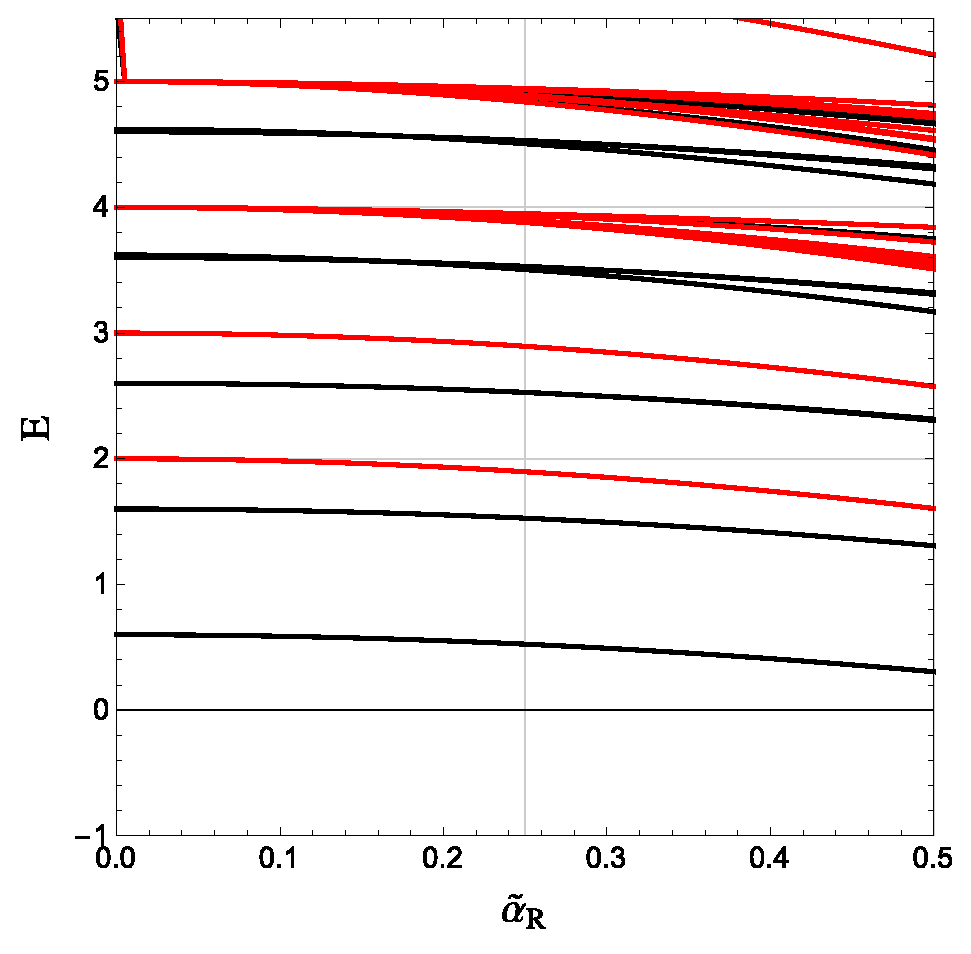
\includegraphics[width=0.5\linewidth]{Figures/Rashbaa1aInf}
\caption{\label{fig:RashbaSpectrum} Spectrum of states with total angular momentum quantum number $J_z=0$ for the Hamiltonian \eqref{eq:RashbaHamiltonian}. The left figure shows the energies without the two-body interaction, i.e. $\tilde{a}=0$ (black), and with negative scattering length $\tilde{a}=-1$ (red). The right figure shows the results for a positive scattering scattering length $\tilde{a}=1$ (black) and in the unitary limit $\tilde{a}\rightarrow\infty$ (red).} 
\end{figure}


Our results for the Rashba SOC are shown in Figure \ref{fig:RashbaSpectrum}. Because the Rashba spin-orbit coupling is a vector operator, states of all possible $J$ must be included in any calculation and the size of the basis scales much more quickly with $E_{max}$. These were computed with an $E_{max}$ of 20, for which we believe the energies convergence to within $0.1\hbar\omega$ for all $a$ over the range of $\alpha_R$ shown. The best convergence is obtained for $a=0$, where the eigenvalues are within $\approx 10^{-5} \hbar \omega$ of the exact values.

\begin{figure}
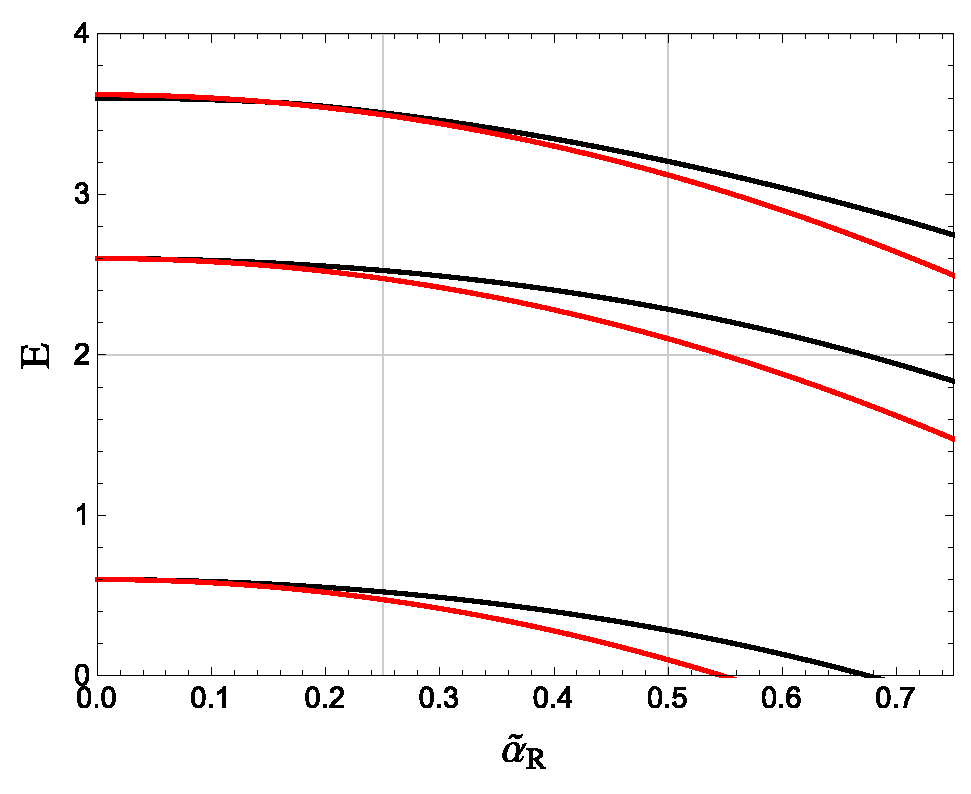
\includegraphics[height=0.4\linewidth]{Figures/ComparisonWithPertap1}
\caption{\label{fig:ComparisonSpectrum} Comparison of selected spectral lines (black) with the perturbative predictions from \cite{PhysRevA.89.033606} (red) when $a=1$. } 
\end{figure}

\begin{figure}
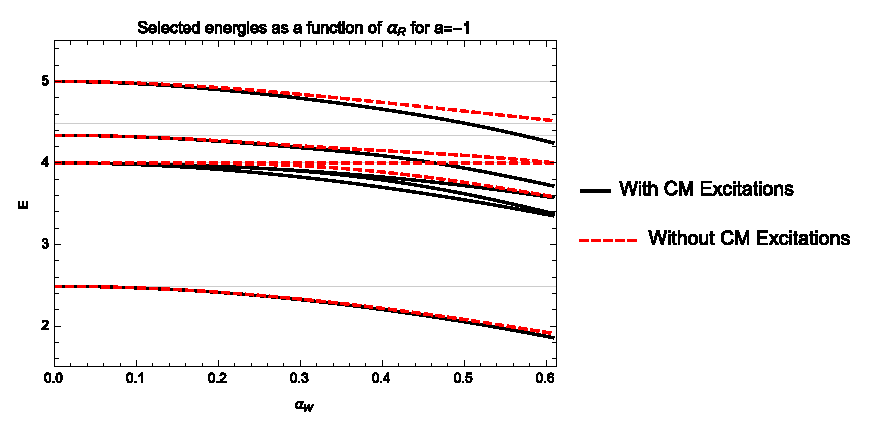
\includegraphics[width=0.9\linewidth]{Figures/NoCMa-1}
\caption{\label{fig:ComparisonSpectrum2} A comparison of the energy levels with and without the inclusion of excitations in the CM coordinate. The approximation of ignoring CM excitations provides very accurate results for the ground state, but not for excited states.} 
\end{figure}


This interaction was also studied perturbatively in $\alpha_R$ by \cite{PhysRevA.89.033606}, including the possibility of a spin dependent two-body interaction, under the assumption that center of mass excitations are unimportant. For the specific case of identical fermions with spin independent scattering length considered here, they found that the first correction to the energies occurs at order $\alpha_R^2$ and is independent of the scattering length $a$. We compare their perturbative predictions with our numerical results in Figure \ref{fig:ComparisonSpectrum}. By setting all matrix elements with $N,L>0$ in the bra or ket to zero, we explored their approximation of ignoring CM excitations. Figure \ref{fig:ComparisonSpectrum2} shows that this is very accurate for the ground state, but less accurate for excited states. We also note that in the case of small positive $a$, the landscape of low lying excited states is dominated by center-of-mass excitations. In the absence of spin-orbit coupling when $a\rightarrow0^+$, there are an infinite number of states with non-zero CM quantum numbers whose energies lie between the ground state and the first relative coordinate excitation.


\section{\label{sec:R=D}Rashba=Dresselhaus SOC}

\begin{figure}
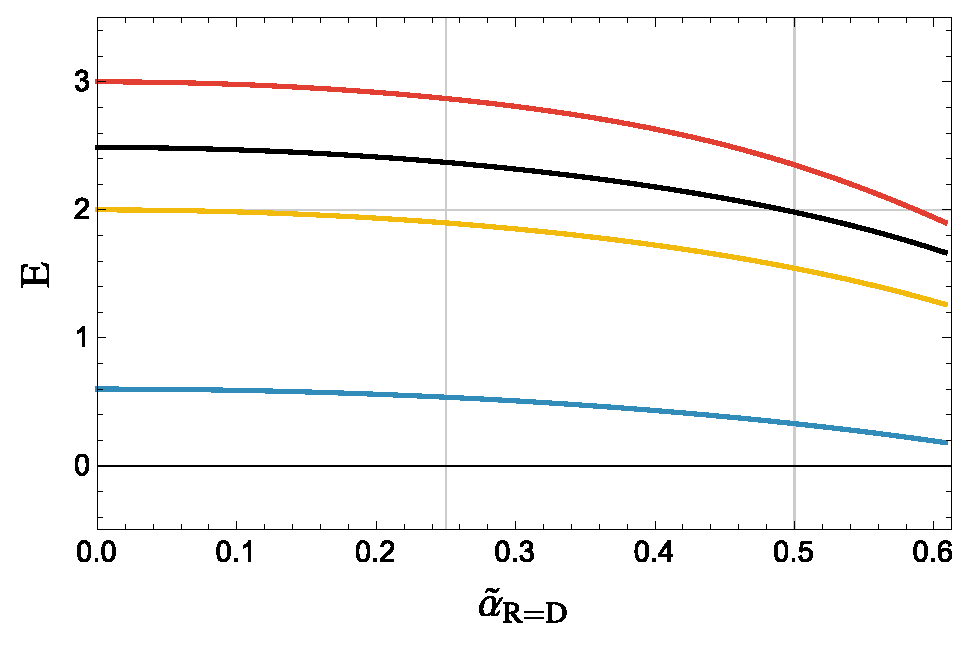
\includegraphics[width=0.65\linewidth]{Figures/R=D_GS}
\caption{\label{fig:R=D_Ground_States} Comparison of the $R=D$ ground state energies for the cases $\tilde{a}=-1$ (black), $\tilde{a}=0$ (red), $\tilde{a}=1$ (blue), $\tilde{a}=\infty$ (orange).} 
\end{figure}

Experiments have thus far only realized the effective Hamiltonian with equal strength Rashba and Dresselhaus couplings in the form \eqref{eq:R=D}. Energy levels of the two-body system in the one-dimensional equivalent of this Hamiltonian with the additional magnetic field couplings present in experimental realizations have been calculated by \cite{guan2014energy}. Here we treat the problem for the first time in three dimensions.

This is also the most computationally difficult of the three cases. When decomposed into spherical tensors, the interaction \eqref{eq:Dresselhaus} becomes
\begin{equation}
V_D=i\,\alpha_D \left( \left[ k \otimes \sigma \right]_{2,-2}- \left[ k \otimes \sigma \right]_{2,2}\right)
\end{equation}
and the two-particle Hamiltonian in the presence of equal strength Rashba and Dresselhaus SOC is given by \eqref{eq:RashbaHamiltonian} with $\alpha_R\rightarrow \alpha_{R=D}$ plus the additional spin-orbit terms
\begin{equation}\label{eq:DresselhausHamiltonian}
\Delta H= \frac{i \tilde{\alpha}_{R=D}}{\sqrt{2}}\left(  \left[ \vec{q} \otimes \vec{\sigma} \right]_{2,-2} -  \left[ \vec{q} \otimes \vec{\sigma} \right]_{2,2} +[ \vec{Q} \otimes \vec{\Sigma} ]_{2,-2} -  [ \vec{Q} \otimes \vec{\Sigma} ]_{2,2} \right).
\end{equation} 
Yet again the number of basis states with nonzero matrix elements has increased; no angular momentum quantum numbers are conserved. The only remaining selection rule will be that the interaction does not change the total magnetic quantum number$J_z$ between even and odd. 

Using the same approach as in the previous sections, the matrix elements of the relative Dresselhaus term are,
\begin{equation}\begin{split}
&\bra{n'(l's')j';N'L';(j'L')J'J'_z} \frac{i \tilde{\alpha}_{R=D}}{\sqrt{2}}\left(  \left[ \vec{q} \otimes \vec{\sigma} \right]_{2,-2} -  \left[ \vec{q} \otimes \vec{\sigma} \right]_{2,2} \right)  \ket{n(ls)j;NL;(jL)JJ_z} = \\
 &\quad\hphantom{\times} i \sqrt{30}(-1)^{J+J'-J'_z+j'+L}\delta_{N,N'}\delta_{L,L'} \sqrt{(2J+1)(2J'+1)(2j+1)(2j'+1)}  \braket{n'l' || q || n l}\\
 &\hspace{1cm}\quad \times(s'-s) \left[\threej{J'}{2}{J}{-J'_z}{-2}{J_z}-\threej{J'}{2}{J}{-J'_z}{2}{J_z}\right] \sixj{j'}{J'}{L}{J}{j}{2}
 \renewcommand{\arraystretch}{0.9} \ninej{\hphantom{l}l'\hphantom{l}}{\hphantom{l}l\hphantom{l}}{\hphantom{l}1\hphantom{l}}{s'}{s}{1}{j'}{j}{2},
\end{split}
\end{equation}
while the center of mass part is,
\begin{equation}\begin{split}
&\bra{n'(l's')j';N'L';(j'L')J'J'_z}  \frac{i \tilde{\alpha}_{R=D}}{\sqrt{2}}\left(  \left[ \vec{Q} \otimes \vec{\Sigma} \right]_{2,-2} -  \left[ \vec{Q} \otimes \vec{\Sigma} \right]_{2,2} \right)  \ket{n(ls)j;NL;(jL)JJ_z} =  \\
&\quad2 i \sqrt{15}(-1)^{J+J'-J'_z+l+1}\delta_{n,n'}\delta_{l,l'}\delta_{s,1}\delta_{s',1}  \\
 &\quad\times \sqrt{(2J+1)(2J'+1)(2j+1)(2j'+1)} \left[\threej{J'}{2}{J}{-J'_z}{-2}{J_z}-\threej{J'}{2}{J}{-J'_z}{2}{J_z}\right] \braket{N' L' || Q || N L} \\ 
 &\quad\times\sum_{\mathcal{J},\mathcal{J}'} (-1)^\mathcal{J}(2\mathcal{J}+1)(2\mathcal{J}'+1)\sixj{l}{1}{j'}{L'}{J'}{\mathcal{J}'}\sixj{l}{1}{j}{L}{J}{\mathcal{J}}\sixj{\mathcal{J}'}{J'}{l}{J}{\mathcal{J}}{2}
 \renewcommand{\arraystretch}{0.9}
 \ninej{\hphantom{l}L'\hphantom{l}}{\hphantom{l}L\hphantom{l}}{\hphantom{l}1\hphantom{l}}{1}{1}{1}{\mathcal{J}'}{\mathcal{J}}{2} .
\end{split}
\end{equation}

The dependence of the lowest energy levels on $\tilde{\alpha}_{R=D}$ for different values of the two-body scattering length is shown in Figure \ref{fig:R=D_Ground_States}. Excitation energies of low lying states are compared in Figure \ref{fig:R=DExcitationSpectrum}.

\begin{figure}
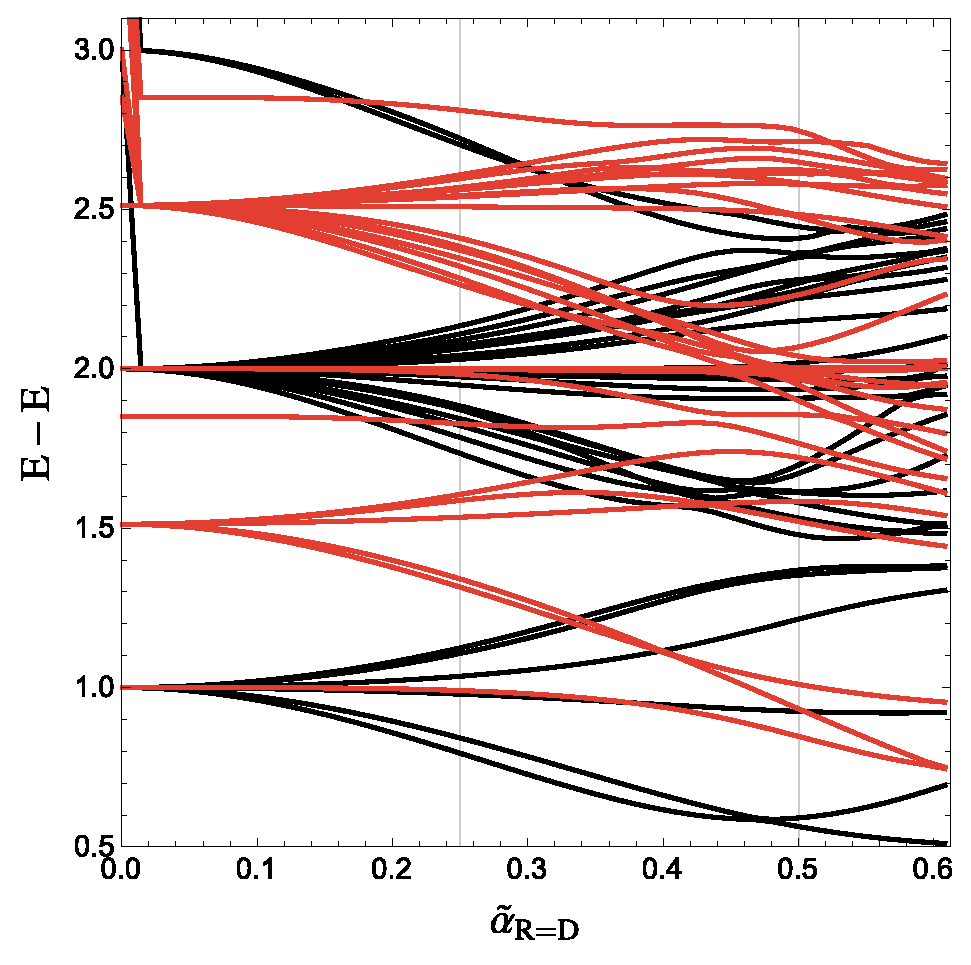
\includegraphics[width=0.5\linewidth]{Figures/R=DExcitation_a0am1}\nobreak
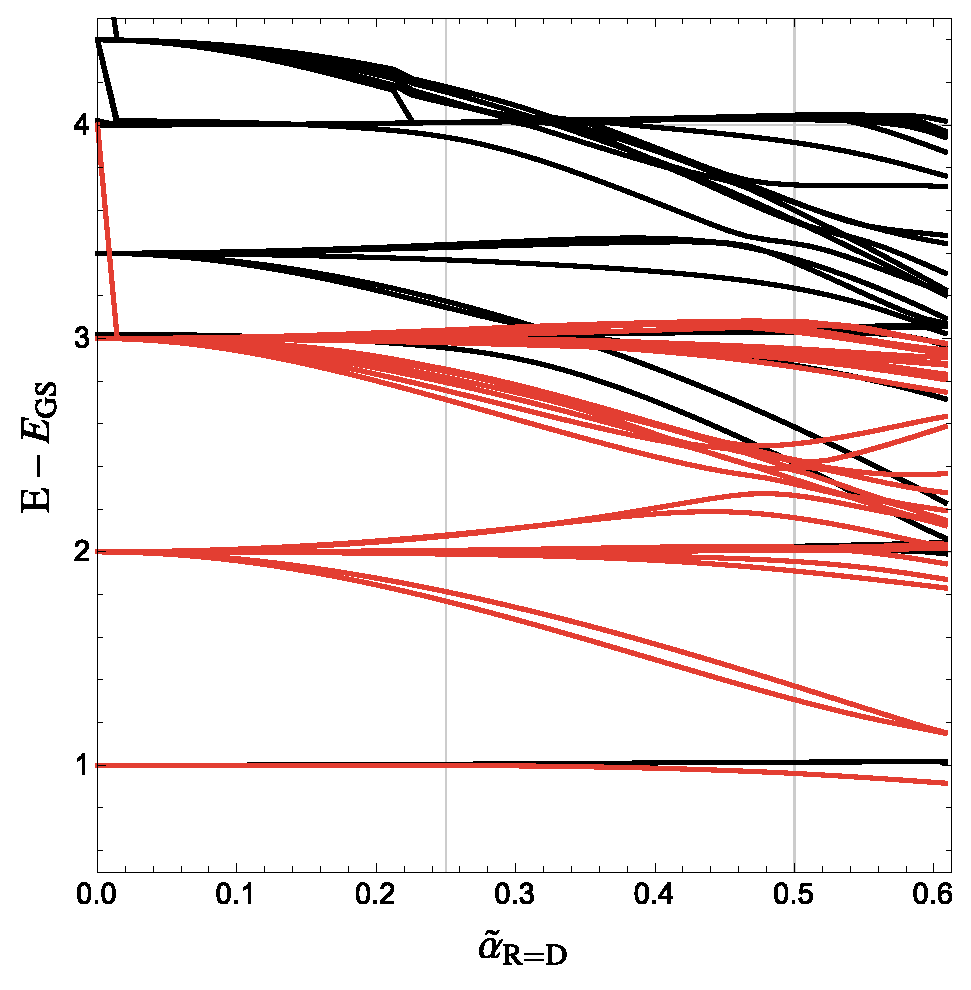
\includegraphics[width=0.5\linewidth]{Figures/R=DExcitation_ap1aInf}
\caption{\label{fig:R=DExcitationSpectrum} Energies relative to the ground state for equal strength Rashba and Dresselhaus spin-orbit couplings. Shown only for states with even $J_z$. The left figure shows the energies without the two-body interaction, i.e. $\tilde{a}_R=0$ (black), and with negative scattering length $\tilde{a}_R=-1$ (red). The right figure shows the results for a positive scattering scattering length $\tilde{a}_R=1$ (black) and in the unitary limit $\tilde{a}_R\rightarrow\infty$ (red).} 
\end{figure}


\section{Conclusions}

We have developed a non-perturbative approach to find the spectrum of two interacting particles in a harmonic trapping potential with spin-orbit coupling. Matrix elements of the Hamiltonian are determined analytically in a basis of the total angular momentum eigenstates of the interacting two-body problem without SOC. With the analytic matrix elements, exact diagonalization within a finite basis is possible.

Our energy calculations are performed in a basis truncated by including all states below a physically meaningful energy cutoff. This approach is effective except in the case where the two-body interaction generates a small, positive scattering length. In this regime coupling of the ground state to higher relative coordinate excited states dominates and convergence in the cutoff parameter $E_{max}$ is numerically intractable. We also observe that although the ground state does not couple strongly to center of mass excitations, their inclusion is crucial for the excited state spectrum. 

Plots of a variety of spectra have been shown for Weyl, Rashba, and equal weight Rashba-Dresselhaus couplings. Although we only have space to show spectra within certain subspaces of conserved angular momentum quantum numbers, the approach presented is fully capable of generating results for all possible states. Larger SO coupling constants are also accessible with larger basis sizes. The general method can easily be adapted to calculate energies for bosonic systems, or to new forms of SOC such as the recently proposed spin-orbital angular momentum coupling \cite{2014arXiv1411.1737S}.


\bibliography{References}

\appendix*
\section{Derivation of the normalization factor for Busch wave functions}
In the original paper by Busch et al \cite{Busch}, the normalization factor of the wave functions is not given. To our knowledge, the closed form expression for this normalization is not widely known. It was originally presented in \cite{PhysRevA.85.053614} without derivation, which we provide here. To find the norm of the wavefunction \eqref{eq:BuschWF}, one must integrate (using a change of variables to $z=r^2$),
\begin{equation}\label{eq:NormIntegral}
A^{-2}=\frac{\Gamma(-n)^2}{8\pi^3}  \int_0^\infty \frac{1}{z}\left[U(-n,3/2,z)e^{-z/2} z^{3/4} \right]^2  dz.
\end{equation}
The terms in brackets is equal to a Whittaker function \cite{DLMF} and so this can be rewritten,
\begin{equation}
A^{-2}=\frac{\Gamma(-n)^2}{8\pi^3}  \int_0^\infty \frac{1}{z}\left[W_{n+3/4,1/4}(z) \right]^2  dz.
\end{equation}
This integral can be found in \cite{GradshteynRyzhik},
\begin{equation}
\int_0^\infty \frac{1}{z}\left[W_{\kappa,\mu}(z) \right]^2  dz=\frac{\pi}{\sin (2\pi \mu)}\frac{\psi_0(\frac{1}{2}+\mu-\kappa)-\psi_0(\frac{1}{2}+\mu-\kappa)}{\Gamma(\frac{1}{2}+\mu-\kappa)\Gamma(\frac{1}{2}-\mu-\kappa)}.
\end{equation}
Applying this to \eqref{eq:NormIntegral} with $\kappa=n+3/4$ and $\mu=1/4$ gives the desired result,
\begin{equation}
A^{-2}=\frac{1}{8\pi^3}  \frac{\Gamma (-n)}{\Gamma(-n-1/2)}\left[\psi(-n)-\psi(-n-1/2)\right]
\end{equation}


\end{document}
%
% ****** End of file apssamp.tex ******
